\documentclass[a4paper, 12pt]{article}
\usepackage[utf8]{inputenc}
\usepackage[portuguese]{babel}

\usepackage{mathptmx}
\usepackage{enumitem}
\usepackage{amsmath}

% Margins
\usepackage{geometry}
\geometry{left=30mm,right=20mm,%
bindingoffset=0mm, top=30mm,bottom=20mm,includefoot}

% Images
\usepackage{graphicx}
\graphicspath{ {./images/} }

% Title font size
\usepackage{titlesec}
\titleformat*{\section}{\bfseries}

% Indent first sentence of a paragraph
\usepackage{indentfirst}

% highlight code
\usepackage{listings}

% Page numbers at bottom right
\usepackage{fancyhdr}
\pagestyle{fancy}
\fancyhf{}
\renewcommand{\headrulewidth}{0pt}
\rfoot{\thepage}

% 1.5 line spacing (yes, 1.25 is actually 1.5)
\fontsize{10}{12}
\linespread{1.50}
\fontfamily{ptm}
\selectfont

% Fix vspacing for section titles
\let\oldsection\section
\renewcommand{\section}[1]{{\vspace{20pt}\oldsection*{#1}\vspace{-10pt}}}

% Indent size
\setlength\parindent{10mm}

% Jump 20pt
\newcommand{\jump}[1]{{\vspace{20pt}}}

\newenvironment{leftquote}[1][]
{
    \hspace{30pt} #1
    \vspace{20pt}
    \fontsize{10}{10}\selectfont
    \begin{flushright}
    \begin{minipage}{120mm}
}
{
    \end{minipage}
    \end{flushright}
    \par
    \vspace{20pt}
}

\newcommand{\tmp}{}

\newenvironment{container}[3]
{
    \renewcommand{\tmp}{#3} %gambiarra
    
    \begin{center}
    \begin{minipage}{#1}
    \centering
    #2
}
{
    \raggedright
    {\footnotesize \tmp}
    \end{minipage}
    \end{center}
}

\begin{document}
	
	% Remove page number
	\clearpage
	\thispagestyle{empty}
	
	\begin{bfseries}
		\begin{center}
			
			
\includegraphics[scale=0.45]{ufc.png} \\
			\vspace{-4pt} 
			UNIVERSIDADE FEDERAL DO CEARÁ \\
			\vspace{4pt} 
			CENTRO DE TECNOLOGIA \\
			\vspace{4pt} 
			DEPARTAMENTO DE TELEINFORMÁTICA \\
			\vspace{4pt}
			\vspace{4pt}
			SEMESTRE 2025.1 \\
			
			
			\vspace*{\fill}
			\textbf{Relatório dos Homeworks de Álgebra Multilinear}
			\vspace*{\fill}
			
		\end{center}
		
		\begin{itemize}[leftmargin=*]
			\setlength{\itemsep}{0pt}
			\item[] ALUNO: Ruan Pereira Alves
			\item[] MATRÍCULA: 569551
		\end{itemize}
		
	\end{bfseries}
	\newpage
	
	\section{Homework 00}
	
	Para o item A
	Geramos aleatoriamente A e B em uma simulação de monte carlo com 1000 etapas. Por conta do custo computacional, foi necessário fazer adaptações a simulação, mais especificamente limitando no item A $n$ a $n \in \{2,4,8,16\}$ e no item B $k$ a $k \in \{2,4,6\}$.
	
	Porém, foi visível no item A a diferença no tempo de compilação entre o método 1 e o método 2, sendo o método 2 muito mais eficiente computacionalmente, por conta do uso da função de inversão em matrizes de dimensão muito menor(a inversão acontece em $N \times N$) do que no método 1(matriz total com dimensão $N^2 \times N^2$)
	
	Para o item a:
	
	\begin{figure}[!h]
		\centering
		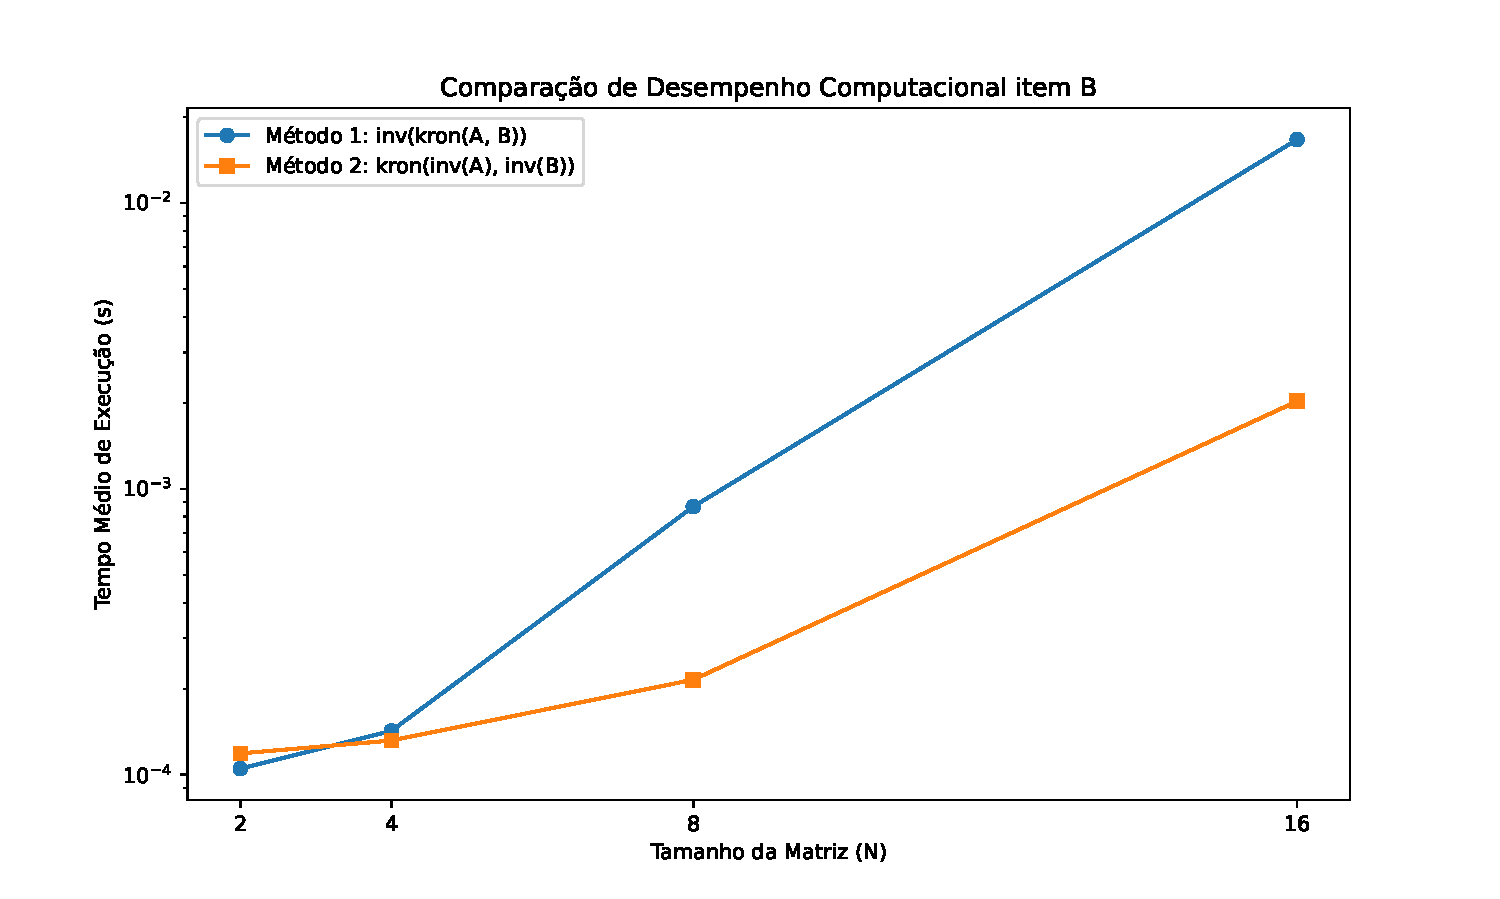
\includegraphics[width=0.9\linewidth]{itema.pdf}
		\caption{Tempo de compilação de acordo com N para cada um dos métodos}
		\label{fig:placeholder}
	\end{figure}
	
	Para o item b: 
	
	\begin{figure}[!h]
		\centering
		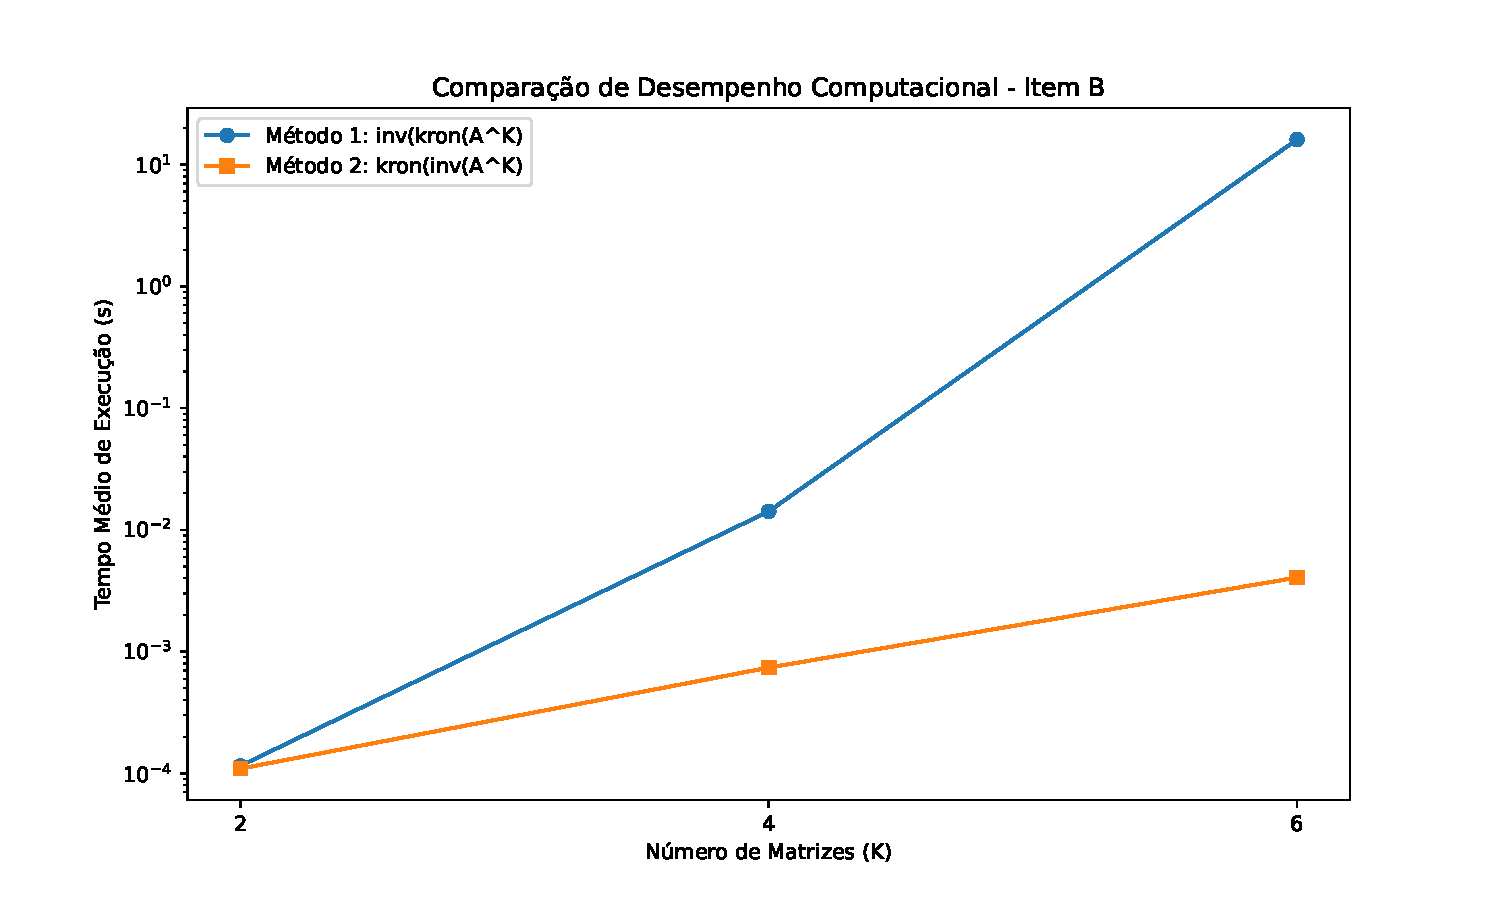
\includegraphics[width=0.9\linewidth]{itemb.pdf}
		\caption{Tempo de compilação de acordo com K para um dos métodos}
		\label{fig:placeholder}
	\end{figure}
	
	\newpage
	
	Para o segundo problema, precisamos encontrar uma forma de mostrar que, se $\lambda$ é $eig(A)$ e $\mu$ é $eig(B)$, então o produto $\lambda\mu$ deve ser equivalente a $eig(A \otimes B)$.
	
	Considerando que $\lambda$ seja um autovalor de A, ele terá um autovetor, que chamaremos de $v$. Assim, teremos que: 
	
	\begin{equation}
		A\mathbf{v} = \lambda \mathbf{v}    
	\end{equation}
	
	Da mesma forma, para B, seja $\mu$ um autovalor de $B$, com $\mathbf{w}$ sendo seu autovetor. Temos:
	
	
	\begin{equation}
		B\mathbf{w} = \mu \mathbf{w}
	\end{equation}
	
	
	Supomos então que o autovetor para $A \otimes B$ seja o produto de Kronecker dos autovetores individuais, ou seja, o vetor $\mathbf{v} \otimes \mathbf{w}$.
	
	Multiplicando ambos, temos: 
	
	
	\begin{equation}
		(A \otimes B)(\mathbf{v} \otimes \mathbf{w})
	\end{equation}
	
	Dai, pelo produto misto:
	
	\begin{equation}
		(A \otimes B)(\mathbf{v} \otimes \mathbf{w}) = (A\mathbf{v}) \otimes (B\mathbf{w})
	\end{equation}
	
	Substituindo a partir da relação encontrada em (1) e (2) no lado direito:
	
	\begin{equation}
		(\lambda \mathbf{v}) \otimes (\mu \mathbf{w})
	\end{equation}
	
	Podemos então retirar os escalares de dentro do produto de Kronecker por propriedade:
	
	\begin{equation}
		\lambda\mu (\mathbf{v} \otimes \mathbf{w})
	\end{equation}
	
	Por fim, temos: 
	
	\begin{equation}
		(A \otimes B)(\mathbf{v} \otimes \mathbf{w}) = (\lambda\mu)(\mathbf{v} \otimes \mathbf{w})
	\end{equation}
	
	o que satisfaz as condições. 
	
	\section{Homework 01}
	
	
	% \section{Homework 09}
	
	% A ideia é decompor um tensor de ordem superior (neste caso, um tensor de terceira ordem $\mathcal{X}$) em uma soma de $R$ componentes de rank-1. Cada componente de rank-1 é o produto externo de $R$ vetores, ou seja o rank do tensor.
	
	% Onde $\mathbf{a}_r$, $\mathbf{b}_r$ e $\mathbf{c}_r$ são os $r$-ésimos vetores das matrizes fatoriais A, B e C, respectivamente, e $\circ$ denota o produto externo. Na prática, isso é equivalente a encontrar as matrizes fatoriais A, B e C.
	
\end{document}

